\documentclass[12pt,a4paper]{article}
\RequirePackage[french]{babel}
\usepackage{fancyhdr}
\usepackage[latin1]{inputenc}
\usepackage{amsfonts}
\usepackage[french]{babel}
\usepackage{listings}
\usepackage{setspace}
\usepackage{graphicx}
\usepackage[T1]{fontenc}
\usepackage{geometry}
\geometry{vmargin=3.5cm,hmargin=2.25cm}
\pagestyle{plain}

\selectlanguage{french}

\begin{document}
\chead{Aegina : rapport de soutenance \no 1}
\begin{titlepage}
\begin{center} 
\huge
\vspace*{5cm}
Aegina : rapport de soutenance \no 1\\
\vspace*{2em}
\large
Florian \bsc{Amsallem} (amsall\_f) , Th�o \bsc{Issarni} (issarn\_t), \\Julien \bsc{Mounier} (mounie\_a), Romain \bsc{Mounier} (mounie\_r)\\
\vspace{2em}
AIM$^{2}$\\
\vspace{2cm}
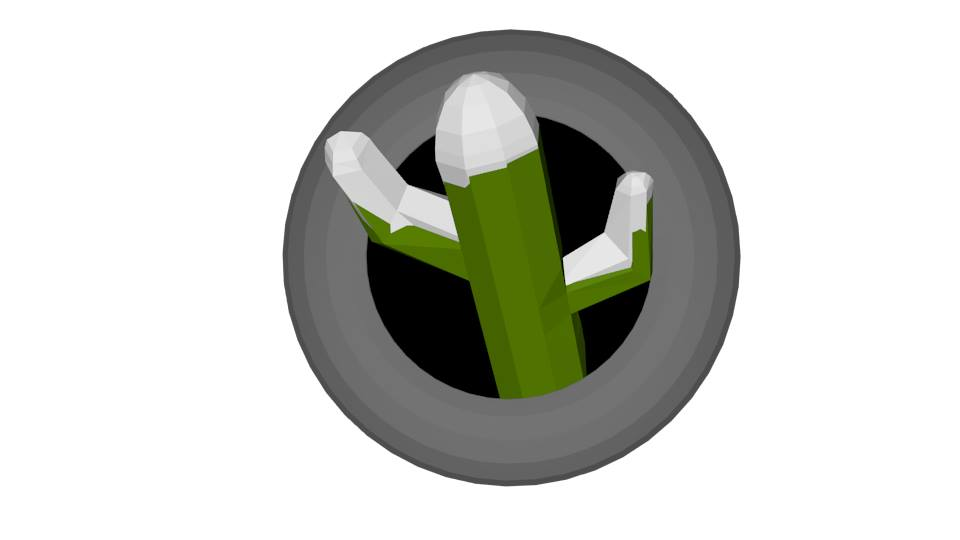
\includegraphics[width=12cm]{logo.jpg}
\end{center} 
\end{titlepage}
\onehalfspacing
\tableofcontents
\pagebreak

\section*{Introduction}
\pagebreak
\addcontentsline{toc}{section}{\protect\numberline{}Introduction}

\section{Univers du jeu}

\subsection{Aegina}

Le monde d'Aegina est constitue d'une casi-infinite d'ile volante. Ce monde ne possede pas de sol, tombe d'une ile engendre une chute sans fin ou du moins c'est ce que l'on suppose. Apres tout personne n'est revenue des trefonds de se monde. Justement ce monde n'est pas tres peuple, seul quelque especes de plante et d'animaux vivent sur ces iles.Cependant on peut y trouver certaine traces de presence humaine notamment en la personne de Ille.

\subsection{Ille}

Ille est le personnqge principale de notre jeux. Il a l'apparence d'un bucheron roux et barbus. En verite Ille n'est pas son vrai nom mais en arrivant dans le monde d'Aegina Ille a perdu la memoire et ne s'en souviens donc plus.

\subsection{Les minerais}

\subsubsection{Mithril}

Le mithril dans le monde d'Aegina et un mineral rose un peu plus solide que le fer. Son interet est sa sensibilite particulieres aux forces etranges qui existe dans Aegina.

\subsubsection{Floatium}

Le floatium et un mineral casi-transparent ayant la capacite d'etre plus leger que l'air. C'est un melange de floatium et de mithril qui est responsable de la levitation des iles de Aeagina.

\subsubsection{sunkium}

Le sunkium et un mineral d'un noir profond qui semble absorber la lumiere. C'est le mineral le plus lourd et le plus dur du monde d'Aegina.
\pagebreak

\section{R�alisation}

\subsection{Pr�-janvier}

\subsubsection{Cycle jour/nuit (Julien)}
Dans un premier temps, on a du d�terminer la dur�e d'une journ�e que l'on a subdiviser en 30 phases. Ces phases servent � changer d'image de skybox. Seulement cette m�thode � caus� quelque probl�mes. Entre autre, le changement de skybox �tait trop brusque et les differentes skybox n'etaient pas homogenes. C'est pourquoi nous avons du trouver une autre methode : La \textit{directional light}.
\\
La \textit{directional light} est un gameobject propose par unity. Son interet majeur est que l'orientation de cette lumiere influance la skybox du monde. De plus nous pouvons choisir la couleur de cette lumiere. Pour ce faire nous avons utilise une fonction qui converti la longueur d'onde des rayons lumineux en couleur RGB et nous avons represente le spectre solaire a l'aide d'une fonction mathematique.
$$255((3.25t - 4)x^2 + (-4t + 4)x)$$
% Mettre un graph de ouf super qui dechire tout !
% TO DO
\subsubsection{Inventaire (Romain et Florian)}
Nous avons creer un inventaire, celui ci est constitue de 24 cases sous forme de 4 lignes et 6 colonnes. Chaque case peut contenir un element, qui peut etre deplacer grace a un drag and drop. De plus le joueur peut avoir une description de chacun des elements en passant sa souris sur celui ci. Cette inventaire s'ouvre lorsaue l'on appui sur la touche \textit{inventaire} qui est de base la touche i et peut ensuite etre ferme avec la touche \textit{inventaire} ou la touche escape. Lorsque l'inventaire est ouvert le joueur et la camera ne peuvent plus bouger 

Lorsque l'inventaire 
\subsubsection{Animation 3D (Th�o)}
Ille est un personnage que nous avons telecharger depuis l'asset store qui possedais de base deux animations, "marcher" et "rester immobile" cependant ces deux seules animation ne nous suffisais pas.
A partir de ce moment nous avons decide de faire les animations des nos personnage nous meme. 
Le premier probleme que nous avons rencontre : notre personnage n'etait pas accessible depuis notre version de blender, trop recente pour le modele 3D aue nous avons. 
Il nous a donc fallut trouver une encienne version de blender compatible avec notre model 3D. Depuis nous essayons d'ameliorer nos animation dans le but d'etre le plus realiste possible.
\subsubsection{D�placement du personnage et de sa camera (Th�o et Julien)}

\subsubsection{Models 3D (Julien)}


\subsection{Janvier}

\subsubsection{Barre de selection (Florian)}

Nous avons ajoute une barre de selection synchronise avec la 4$^{eme}$ ligne de notre inventaire. De plus le joueur peut selectionner une case de cette barre et utiliser l'objet s'y trouvant. Cette barre apparait meme quand le joueur n'est pas dans son inventaire

\subsubsection{Menus (Romain et Florian)}

Nous avons cree des menus  permetant de modifier la langue et le volume du son du jeu. Ces menus s'ouvre avec la touche escape quand aucune autre interface n'est ouvert et ce ferme avec la touche escape ou avec le bouton \textit{continuer}. Dans le menu le joueur et la camera du joueur ne peuvent pas bouger comme lorsque l'inventaire et ouvert.

\subsubsection{Class \textit{Item} (Romain)}

Dans l'inventaire nous voulons parfois des objets en grandes quantite nous avons alors cree des classes \textit{Item} et \textit{Itemstack} 

\subsubsection{Multi-joueurs (Florian)}

\subsubsection{Son (Th�o et Romain)}


\subsection{F�vrier}

\subsubsection{G�n�ration al�atoire (Florian et Julien)}

\subsubsection{Drop d'Item (Florain et Julien)}

\subsubsection{Biblioth�que (Florian, Romain et Th�o)}

\subsubsection{Histoire (Romain et Th�o)}


\subsection{Mars}

\subsubsection{Int�raction avec l'environnement (Florian et Julien)}

\subsubsection{Cristal (Romain et Julien)}

\subsubsection{Chat (Florian)}

\subsubsection{Musique (Th�o)}

\subsubsection{Survie (Th�o)}

\subsubsection{Alpha (Florian)}

\pagebreak

\section{Pr�vision}

\subsection{Les quatre grand axe}

\subsubsection{Creation d'objet}

\subsubsection{Ajout des cr�atures}

\subsubsection{Ajout des succ�s}

\subsubsection{PVP et Conqu�te}


\subsection{Les am�liorations}

\subsubsection{Survie}

\subsubsection{G�n�ration al�atoire et sauvegarde}

\subsubsection{Histoire}

\subsubsection{Environnement sonore}

\subsubsection{Personnage}

\pagebreak

\section*{Conclusion}
\addcontentsline{toc}{section}{\protect\numberline{}Conclusion}
\end{document}
